\chapter{Main Results and Robustness Checks}

\section{Main Result: Reviewed Banglish Remains Harder}

Table~\ref{tab:main-v5} gives the main frozen validation-200 v5 result.

\begin{table}[H]
\centering
\caption{Main validation-200 v5 results}
\label{tab:main-v5}
\small
\resizebox{\textwidth}{!}{%
\begin{tabular}{llllll}
\hline
Model & Bangla & Reviewed Banglish & English & Banglish - Bangla & Banglish - English \\
\hline
Qwen2.5-3B & 54/200 & 41/200 & 71/200 & -6.5 pts, CI [-13.0, 0.0] & -15.0 pts, CI [-22.0, -7.5] \\
Qwen2.5-7B 8-bit & 65/200 & 47/200 & 94/200 & -9.0 pts, CI [-16.0, -2.0] & -23.5 pts, CI [-31.0, -16.0] \\
Qwen3-4B & 80/200 & 49/200 & 88/200 & -15.5 pts, CI [-22.0, -9.0] & -19.5 pts, CI [-27.0, -12.0] \\
\hline
\end{tabular}%
}
\end{table}

The result is consistent across the three thesis-facing Qwen models. Reviewed Banglish is lower than native-script Bangla and English for every model. Qwen2.5-7B and Qwen3-4B have fully negative Banglish-minus-Bangla confidence intervals. Qwen2.5-3B has a negative point estimate but the all-200 interval touches zero. This is why the claim must be stated carefully: the strongest all-200 evidence comes from Qwen2.5-7B and Qwen3-4B, while Qwen2.5-3B remains supportive through point estimate, historical v3 results, and strict-197 sensitivity.

The English comparison is larger. For all three Qwen rows, reviewed Banglish is 15 to 23.5 points below English. This supports the idea that many failures are not simply item difficulty. The same item can become answerable when shown in a different script or language view.

Figure~\ref{fig:paired-gaps} shows the same pattern visually, together with the frontier/API panel from Chapter~\ref{chap:frontier}: reviewed Banglish is the lowest bar for every model except GPT-5.5, and the Banglish-minus-Bangla interval excludes zero for seven of the eight models.

\begin{figure}[H]
\centering
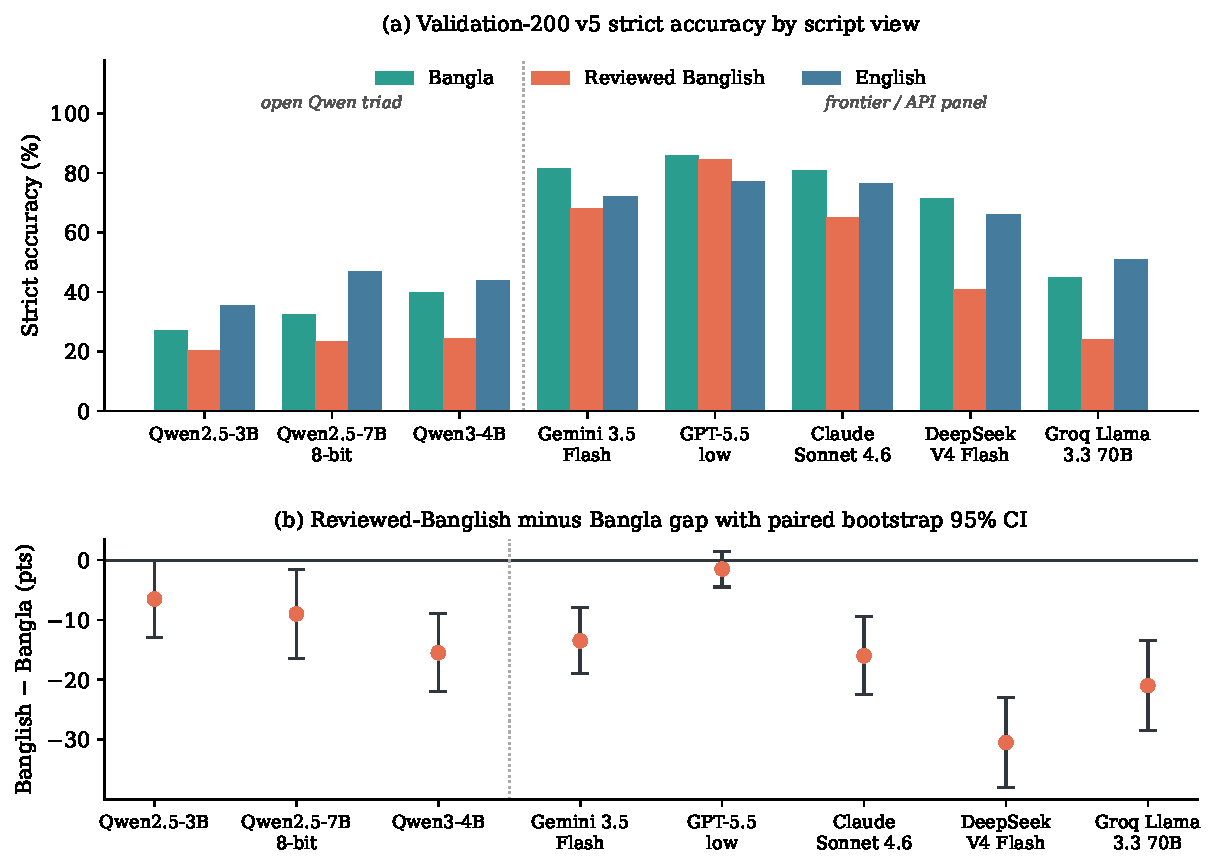
\includegraphics[width=\textwidth]{figures/fig_paired_gaps.pdf}
\caption{Validation-200 v5 strict accuracy by script view (top) and the reviewed-Banglish minus Bangla gap with paired bootstrap 95\% confidence intervals (bottom) for the open Qwen triad and the five-model frontier/API panel.}
\label{fig:paired-gaps}
\end{figure}

\section{Exact Paired Significance: McNemar Tests}

The paired design is the textbook McNemar setting: each item produces a paired binary outcome under two prompt scripts. The exact McNemar test uses only the discordant pairs --- items where exactly one script view is correct --- so it is insensitive to the large mass of items that both views answer identically. We report the discordant counts ($b$ = Bangla-only correct, $c$ = Banglish-only correct), the exact two-sided p-value, the conditional odds ratio $b/c$ with a Haldane-corrected 95\% interval, and Holm-adjusted p-values across the three models.

\begin{table}[H]
\centering
\caption{McNemar exact tests for reviewed Banglish versus Bangla on validation-200 v5. $b$ counts Bangla-only-correct items; $c$ counts Banglish-only-correct items.}
\label{tab:mcnemar-qwen}
\small
\begin{tabular}{lrrlll}
\hline
Model & $b$ & $c$ & Odds ratio [95\% CI] & Exact $p$ & Holm $p$ \\
\hline
Qwen2.5-3B & 28 & 15 & 1.84 [0.99, 3.41] & 0.066 & 0.066 \\
Qwen2.5-7B 8-bit & 37 & 19 & 1.92 [1.11, 3.32] & 0.022 & 0.044 \\
Qwen3-4B & 39 & 8 & 4.65 [2.22, 9.75] & $<$0.0001 & $<$0.0001 \\
\hline
\end{tabular}%
\end{table}

The exact tests sharpen the bootstrap story. Qwen3-4B and Qwen2.5-7B remain significant after Holm correction. Qwen2.5-3B is marginal on the 200-item core ($p = 0.066$), which matches its CI-touches-zero bootstrap interval; on the 974-row BEnQA extension in Chapter~\ref{chap:frontier}, the same model's Bangla-versus-Banglish contrast becomes significant ($p = 0.024$), confirming that the marginal core result reflects sample size rather than absence of effect. The Banglish-versus-English contrasts are exact-test significant for all three models ($p \leq 0.0001$). Full tables for all panels, including the API panel and the extension, are in \url{https://github.com/munimthahmid/BanglishBench/blob/main/reports/mcnemar_script_gaps.md}.

\section{Per-Task Breakdown: BEnQA versus BanglaMATH}

The two source tasks contribute differently to the aggregate result, so Table~\ref{tab:per-task} splits the main result by task.

\begin{table}[H]
\centering
\caption{Validation-200 v5 results split by source task. Gaps are reviewed Banglish minus Bangla with paired bootstrap 95\% CIs.}
\label{tab:per-task}
\small
\resizebox{\textwidth}{!}{%
\begin{tabular}{llllll}
\hline
Task & Model & Bangla & Reviewed Banglish & English & Banglish -- Bangla \\
\hline
BEnQA (144) & Qwen2.5-3B & 49/144 & 41/144 & 66/144 & -5.6 pts, CI [-13.9, +2.8] \\
BEnQA (144) & Qwen2.5-7B 8-bit & 60/144 & 47/144 & 86/144 & -9.0 pts, CI [-18.8, +0.7] \\
BEnQA (144) & Qwen3-4B & 76/144 & 47/144 & 82/144 & -20.1 pts, CI [-28.5, -11.8] \\
BanglaMATH (56) & Qwen2.5-3B & 5/56 & 0/56 & 5/56 & -8.9 pts, CI [-17.9, -1.8] \\
BanglaMATH (56) & Qwen2.5-7B 8-bit & 5/56 & 0/56 & 8/56 & -8.9 pts, CI [-16.1, -1.8] \\
BanglaMATH (56) & Qwen3-4B & 4/56 & 2/56 & 6/56 & -3.6 pts, CI [-8.9, 0.0] \\
\hline
\end{tabular}%
}
\end{table}

The BEnQA subset carries the cleanest evidence, as anticipated in Chapter 3: choice-label scoring is insensitive to answer formatting, and the Qwen3-4B BEnQA gap is the largest and most precisely estimated single contrast in the core ($-20.1$ points). The BanglaMATH subset operates near the strict-scoring floor --- the compact Qwen models answer almost no Banglish math item in deployable form --- so its gaps are smaller in absolute points but reflect a complete loss of usable accuracy under Banglish input. The two tasks therefore tell complementary stories: BEnQA measures a graded semantic gap, while BanglaMATH shows strict answer compliance collapsing under script change.

\section{Review Sensitivity}

A natural first objection is that the Latin-script Banglish field might simply be bad Banglish. The v5 review was designed to test that possibility. It targeted rows where review could matter most, then froze the final validation-200 slice. The result is clear: review changes scores only slightly and does not remove the gap.

This matters for interpretation. If Banglish cleanup had raised scores to match Bangla, the result would mostly be about romanizer artifacts. Instead, cleanup improves quality while preserving the central pattern. The study therefore does not need to claim that every romanization is perfect. It only needs to show that the observed gap is not removed by targeted review.

We also report what happens when the three flagged source-quality rows are excluded. Under this strict-197 policy, the reviewed Banglish-minus-Bangla intervals remain negative for all three thesis-facing Qwen rows:

\begin{table}[H]
\centering
\caption{Strict-197 sensitivity check after excluding three flagged source-quality rows.}
\label{tab:strict197}
\small
\begin{tabular}{lll}
\hline
Model & Strict policy & Reviewed Banglish - Bangla \\
\hline
Qwen2.5-3B & 197 rows & -7.1 pts, CI [-13.2, -1.0] \\
Qwen2.5-7B 8-bit & 197 rows & -9.6 pts, CI [-16.8, -2.5] \\
Qwen3-4B & 197 rows & -15.7 pts, CI [-22.3, -9.6] \\
\hline
\end{tabular}%
\end{table}

The strict-197 view is not the primary denominator. It is a check that the main result does not depend on a few questionable rows.

\section{Tokenization Sensitivity}

Another plausible explanation is tokenization. If Banglish were much longer than Bangla, lower accuracy could be a context-budget or tokenization-efficiency problem. The data do not support that simple explanation.

For the audited Qwen tokenizers, reviewed Banglish is token-cheaper than native Bangla.

\begin{table}[H]
\centering
\caption{Mean tokens per word under the audited Qwen tokenizers}
\label{tab:tokens-per-word}
\small
\begin{tabular}{llll}
\hline
Dataset & Bangla & Reviewed Banglish & English \\
\hline
BEnQA & 4.02 & 2.49 & 1.95 \\
BanglaMATH & 4.63 & 2.11 & 1.41 \\
\hline
\end{tabular}%
\end{table}

Figure~\ref{fig:token-cost} makes the point visually: for every Qwen model, the reviewed-Banglish point sits to the left of the Bangla point (cheaper in tokens per word) and below it (less accurate). Token cost and accuracy are decoupled across scripts.

\begin{figure}[H]
\centering
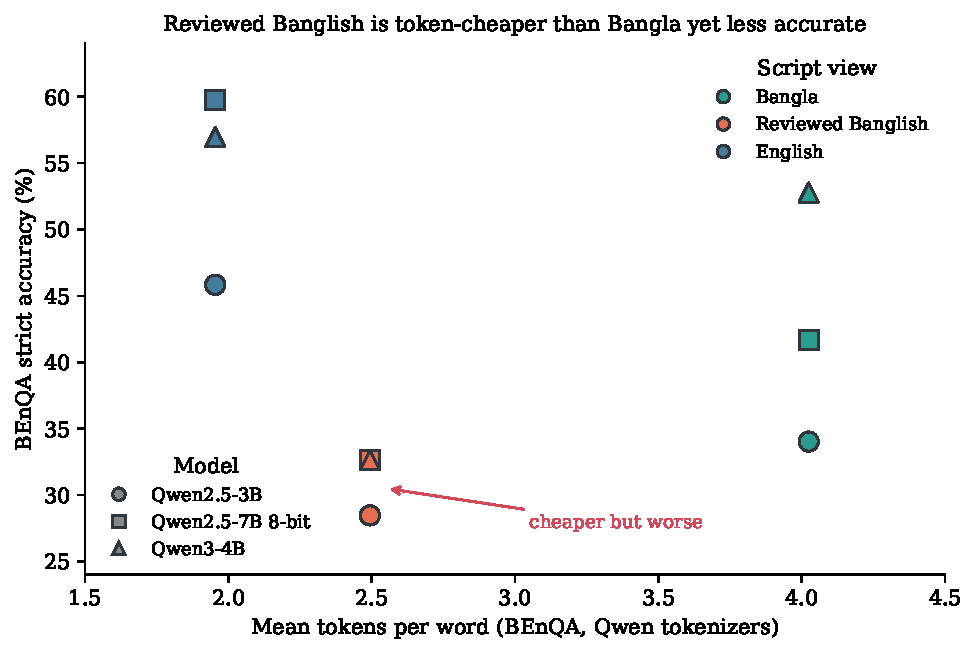
\includegraphics[width=0.82\textwidth]{figures/fig_token_cost.pdf}
\caption{Token cost versus BEnQA strict accuracy for the Qwen triad on validation-200 v5. Reviewed Banglish costs fewer tokens per word than native Bangla under the audited Qwen tokenizers, yet is less accurate for every model.}
\label{fig:token-cost}
\end{figure}

The failure-pattern join also shows that recoverable Banglish misses are not the longest Banglish prompts. In BEnQA, recoverable reviewed-Banglish misses are shorter on average than other rows for all three thesis-facing Qwen models.

This does not prove tokenization is irrelevant. Tokenization can affect representation quality in ways not captured by length. But it rules out the simple explanation that Banglish fails because it uses more tokens. The failure is more consistent with script-conditioned lexical grounding, training distribution, spelling variation, and task interpretation.

\section{Prompt and Decoding Sensitivity}

A remaining objection is that the gap is an artifact of one prompt template or greedy decoding. We test this by rerunning Qwen2.5-3B on validation-200 v5 under two neutral alternate prompt templates --- one terse, one exam-role-framed, neither containing any Banglish hint --- and a temperature-0.7 decoding variant.

\begin{table}[H]
\centering
\caption{Prompt and decoding sensitivity for Qwen2.5-3B on validation-200 v5. The Banglish-minus-Bangla gap stays negative across all conditions.}
\label{tab:prompt-sensitivity}
\small
\begin{tabular}{lllll}
\hline
Condition & Bangla & Banglish & English & Banglish -- Bangla \\
\hline
Baseline (greedy) & 54/200 & 41/200 & 71/200 & -6.5 pts \\
Neutral template B (terse) & 51/200 & 45/200 & 71/200 & -3.0 pts \\
Neutral template C (exam role) & 53/200 & 45/200 & 74/200 & -4.0 pts \\
Temperature 0.7 & 53/200 & 44/200 & 71/200 & -4.5 pts \\
\hline
\end{tabular}%
\end{table}

The Banglish-minus-Bangla gap stays negative ($-3.0$ to $-6.5$ points) under every template and the temperature change, and the Banglish-minus-English gap stays large ($-13.0$ to $-15.0$ points). The effect is therefore not produced by a particular instruction wording or by greedy decoding; it survives the same way the review, strict-197, and tokenization checks survive.

\section{Spelling-Variation Robustness}

The clearest stated limitation of the controlled benchmark is that one rule-based romanizer is not natural, spelling-variable Banglish. We test whether the script penalty depends on the specific spelling by generating, for a 100-item BEnQA subset, four additional seeded phonetic respellings of each item's reviewed Banglish (substitutions such as \texttt{sh}$\rightarrow$\texttt{s}, \texttt{bh}$\rightarrow$\texttt{v}, \texttt{kichhu}$\rightarrow$\texttt{kichu}), preserving digits, formulae, option labels, and the answer line. Each item is then answered under all five spellings.

\begin{table}[H]
\centering
\caption{Correctness stability across five Banglish spellings of the same 100 BEnQA items. A flip is an item whose correctness is not constant across spellings.}
\label{tab:spelling}
\small
\begin{tabular}{lrrrrr}
\hline
Model & Accuracy & Spelling range & Items flipping & Flip rate & Mean swing \\
\hline
Qwen2.5-3B & 31.2\% & 28--34\% & 17/100 & 17\% & 0.17 \\
Qwen3-4B & 29.0\% & 28--31\% & 6/100 & 6\% & 0.06 \\
\hline
\end{tabular}%
\end{table}

Two findings emerge, and they point in complementary directions. First, the \emph{magnitude} of Banglish accuracy is stable across independent spellings: per-spelling accuracy stays in a narrow 28--34\% band for both models, so the script penalty is not an artifact of one particular romanizer's spelling choices. This directly addresses the naturalness limitation. Second, at the \emph{item} level, robustness is not perfectly stable: 17\% of items for Qwen2.5-3B (and 6\% for Qwen3-4B) flip correctness when only the spelling changes, with the gold answer and question fixed. Banglish reliability is therefore both systematically lower and locally unstable under realistic spelling variation --- the same user question can be answered or missed depending on how it happens to be romanized.

\endinput
